\documentclass[10pt,a4paper]{article}
\usepackage[utf8]{inputenc}
\usepackage{amsmath}
\usepackage{amsfonts}
\usepackage{amssymb}
\usepackage{graphicx}
\author{Marcelo Lynch}
\usepackage[margin=1.2in]{geometry}


\newcommand{\N}{\mathbb{N}}
\newcommand{\Z}{\mathbb{Z}}
\newcommand{\Q}{\mathbb{Q}}
\newcommand{\R}{\mathbb{R}}
\newcommand{\C}{\mathbb{C}}
\newcommand{\Rr}{\mathcal{R}}
\newcommand{\G}{\Gamma}
\newcommand{\ra}{\rightarrow}
\newcommand{\bra}{\textcolor{blue}{\longrightarrow}}
\newcommand{\bla}{\textcolor{blue}{\longleftarrow}}
\newcommand{\rra}{\textcolor{red}{\longrightarrow}}
\newcommand{\rla}{\textcolor{red}{\longleftarrow}}
\newcommand{\Ra}{\Rightarrow}
\renewcommand{\S}{\Sigma}
\newcommand{\bz}{\bm{0}}
\newcommand{\bo}{\bm{1}}

\newcommand{\peq}{\preceq}

\renewcommand{\a}{\alpha}
\renewcommand{\b}{\beta}
\newcommand{\g}{\gamma}

\renewcommand{\L}{\mathcal{L}}
\newcommand{\I}{\mathcal{I}}
\newcommand{\genericfol}{\L = (\mathcal{F})}
\newcommand{\U}{\mathcal{U}}

\title{\vspace{-1.6cm}Visualizando $c^{\aleph_0} = (2^{\aleph_0})^{\aleph_0} = 2^{\aleph_0 \cdot \aleph_0} = 2^{\aleph_0} = c$ }
\author{Marcelo Lynch}
\date{}
\begin{document}

\maketitle

Sabiendo que $(a^b)^c = a^{b \cdot c}$, que $\aleph_0 \cdot \aleph_0 = \aleph_0$ y $c = 2^{\aleph_0}$, es inmediato ver que \[ c^{\aleph_0} = (2^{\aleph_0})^{\aleph_0} = 2^{\aleph_0 \cdot \aleph_0} = 2^{\aleph_0} = c \]. Otra manera de escribir esto es:

\[ (0,1)^\N \sim (\{0, 1\}^\N)^{\N} \sim \{ 0,1 \}^{\N \times \N} \sim \{0,1\}^\N \sim (0,1) \]

Es ilustrativo\footnote{En el fondo no vamos a estar haciendo nada nuevo, únicamente ``componer'' las demostraciones individuales de $(a^b)^c = a^{b \cdot c}$, $\aleph_0 \cdot \aleph_0 = \aleph_0$ y $c = 2^{\aleph_0}$, pero quizás es interesante verlo en un ejemplo concreto} ver una manera ``natural'' de relacionar los elementos de estos conjuntos para convencerse de que de alguna manera ``son lo mismo'', y es lo que vamos a hacer \textbf{(informalmente)} a continuación.  La idea va a ser mostrar como \textbf{un elemento particular} del conjunto $(0,1)^\N$ \textit{``puede pensarse como''} un elemento de cualquiera de los otros conjuntos.\\

Partimos entonces de un elemento $a \in (0,1)^{\N}$. Esta $a$ es una función de $\N$ al intervalo $(0,1)$, es decir una sucesión de numeros reales de ese intervalo. O sea que $a$ es una \textit{lista infinita de numeros reales} $a_0, a_1, a_2, \cdots$. Si escribimos cada uno de estos números en binario (y supongamos, en la escritura sin colas de $1$), podemos hacer una lista con todos los elementos uno abajo del otro así:

\[ 0,a_0^0\ a_0^1\ a_0^2\ a_0^3\ a_0^4\ \cdots \]
\[ 0,a_1^0\ a_0^1\ a_1^2\ a_1^3\ a_1^4\ \cdots \]
\[ 0,a_2^0\ a_0^1\ a_2^2\ a_2^3\ a_2^4\ \cdots \]
\[ 0,a_3^0\ a_0^1\ a_3^2\ a_3^3\ a_3^4\ \cdots \]
\[ 0,a_4^0\ a_0^1\ a_4^2\ a_4^3\ a_4^4\ \cdots \]
\[\ \ \vdots\ \hspace{30px}  \hspace{30px} \]
Donde $a_i^j$ es el $j$-ésimo dígito (despues de la coma) del numero $a_i$, y siempre es $0$ o $1$.\\

Estos números siempre se van a poder escribir como ``cero coma algo'', porque están en $(0,1)$, entonces podemos ahorrarnos escribir eso y solamente identificar a cada numero con la parte después de la coma. Si además numeramos cada fila con un número natural, y ``separamos los dígitos'', nos queda:

\[ 0 \ra a_0^0,\ a_0^1,\ a_0^2,\ a_0^3,\ a_0^4,\ \cdots \]
\[ 1 \ra a_1^0,\ a_0^1,\ a_1^2,\ a_1^3,\ a_1^4,\ \cdots \]
\[ 2 \ra a_2^0,\ a_0^1,\ a_2^2,\ a_2^3,\ a_2^4,\ \cdots \]
\[ 3 \ra a_3^0,\ a_0^1,\ a_3^2,\ a_3^3,\ a_3^4,\ \cdots \]
\[ 4 \ra a_4^0,\ a_0^1,\ a_4^2,\ a_4^3,\ a_4^4,\  \cdots \]
\[\ \ \vdots\ \hspace{50px} \vdots\ \vdots\ \vdots \hspace{50px} \]

¡Momento! A cada número natural (el numero de la fila) le podemos asignar una lista infinita de dígitos $0$ y $1$. Pero eso es lo mismo que asignarle una sucesión de $0$ y $1$ a cada numero natural: ¡este dibujo es el de una función $\N \ra \{0, 1\}^\N$! Entonces otra manera de ``distribuir'' la información de $a$ es en un elemento de $(\{0, 1\}^\N)^\N$. Pero podemos ir más allá: en vez de solamente ponerle número a las filas, podemos también numerar las columnas:


\[\ \ \ \ \ \ \ 0\ \ \ \ 1\ \ \ \ 2\ \ \ \ 3\ \ \ \ 4\cdots \]
\[\ \ \ \ \ \ \ \downarrow\ \ \ \ \downarrow\ \ \ \ \downarrow\ \ \ \ \downarrow\ \ \ \downarrow\ \ \  \]
\[ 0\  \ra\  a_0^0\ \ a_0^1\ \ a_0^2\ \ a_0^3\ \ a_0^4\  \cdots \]
\[ 1\  \ra\  a_1^0\ \ a_1^1\ \ a_1^2\ \ a_1^3\ \ a_1^4\  \cdots \]
\[ 2\  \ra\  a_2^0\ \ a_2^1\ \ a_2^2\ \ a_2^3\ \ a_2^4\  \cdots \]
\[ 3\ \ra\ a_3^0\ \ a_3^1\ \ a_3^2\ \ a_3^3\ \ a_3^4\  \cdots \]
\[ 4\ \ra\  a_4^0\ \ a_4^1\ \ a_4^2\ \ a_4^3\ \ a_4^4\  \cdots \]
\[\ \ \vdots\ \hspace{50px} \vdots\ \vdots\ \vdots \hspace{50px} \]


Y entonces podemos pensar este dibujo como una asignación de $0$ o $1$ a cada coordenada $(i, j)$ donde $i$ es la fila y $j$ la columna: pero esto es precisamente una función $\N \times \N \ra \{0, 1\}$, o sea un elemento de $\{0, 1\}^{\N \times \N}$.\\ 


Ahora, ¿cómo hacemos para transformar esto en una única sucesión de ceros y unos (o sea, un elemento de $\{ 0, 1 \}^\N$? El truco  está en recorrer la ``cuadrícula'' de manera tal de no perdernos ninguno, y asi armar la sucesión individual:

\begin{figure}[h!]
\centering
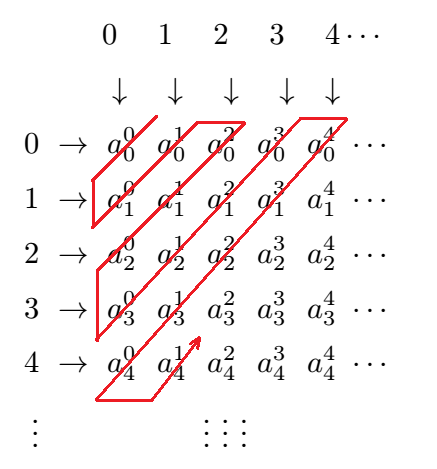
\includegraphics[scale=0.9]{diagonales.png}
\end{figure}

Haciendo este zigzag podemos ir \textbf{recorriendo todos los dígitos sin saltearnos ninguno}. Con este recorrido podemos armar la sucesión: 
\[ a_0^0,\ a_1^0,\ a_0^1, \ a_0^2,\ a_1^1,\ a_2^0, \ \cdots \]

¡Y ya está! Toda la tabla de infinitas filas e infinitas columnas nos queda condensada \textit{en una sola sucesión} de ceros y unos. Por como elegimos la representacion de los números al principio, esta sucesión tampoco tendrá colas de $1$. Notemos que dada una de estas sucesiones podemos reconstruir la tabla, si la arrancamos vacía y vamos llenando los espacios mientras recorremos con el mismo zig-zag, es decir, no se pierde información. \\


Finalmente, la manera de transformar esta sucesión en un único número real es usando los elementos como dígitos en la representación binaria (sin colas de $1$) del número:

\[ x = 0,a_0^0\ a_1^0\ a_0^1 \ a_0^2\ a_1^1\ a_2^0 \ \cdots \]



\ \\
\textbf{\underline{Observación}}: Cada una de estas operaciones que fuimos haciendo puede pensarse como una función que lleva un elemento de un conjunto a un elemento del siguiente. Como estuvimos forzados a eliminar representaciones al principio, estas construcciones no constituyen biyecciones, o sea, hay algunos elementos de $(\{0,1 \}^\N)^\N$ que no podríamos construir cuando hacemos el primer paso desde $(0,1)^\N$. Pero sí son inyecciones, porque todas las construcciones son reversibles. 

\end{document}